%----------------------------------------------------------------------------------------
%	PACKAGES AND OTHER DOCUMENT CONFIGURATIONS
%----------------------------------------------------------------------------------------
\documentclass[11pt,a4paper]{article}

\usepackage[utf8]{inputenc} % to encode the document so that we can use more caracters (like Latin ones)
\usepackage[T1]{fontenc} % to encode the document so that we can use more caracters (like Latin ones)
\usepackage[english]{babel} % to write in English

\usepackage{geometry} % the paper's format and marges
\geometry{hmargin=2.3cm,vmargin=1.7cm}

\usepackage{titling} % to put the title where I want

% maths packages
\usepackage{mathtools}
\usepackage{amsmath,amsbsy}
\usepackage{bm}
\usepackage{bigints}
\usepackage{stmaryrd}
\usepackage{amsfonts}

% graphs packages
\usepackage{graphicx}
\usepackage{float}
\usepackage{caption}
\usepackage{subcaption}
\usepackage{wrapfig,epsfig}

\usepackage{color}

\newtheorem{theorem}{Theorem}[section]
\newtheorem{lemma}[theorem]{Lemma}
\newtheorem{proposition}[theorem]{Proposition}
\newtheorem{corollary}[theorem]{Corollary}

\newenvironment{proof}[1][Proof]{\begin{trivlist}
		\item[\hskip \labelsep {\bfseries #1}]}{\end{trivlist}}
\newenvironment{definition}[1][Definition]{\begin{trivlist}
		\item[\hskip \labelsep {\bfseries #1}]}{\end{trivlist}}
\newenvironment{example}[1][Example]{\begin{trivlist}
		\item[\hskip \labelsep {\bfseries #1}]}{\end{trivlist}}
\newenvironment{remark}[1][Remark]{\begin{trivlist}
		\item[\hskip \labelsep {\bfseries #1}]}{\end{trivlist}}

\newcommand{\qed}{\nobreak \ifvmode \relax \else
	\ifdim\lastskip<1.5em \hskip-\lastskip
	\hskip1.5em plus0em minus0.5em \fi \nobreak
	\vrule height0.75em width0.5em depth0.25em\fi}

\usepackage{vmargin}
\setmarginsrb{0.5cm}{0.5cm}{1cm}{1cm}{0cm}{0cm}{0cm}{0cm}

\usepackage[final]{pdfpages}

\usepackage{algorithm}
\usepackage{algorithmic}
%----------------------------------------------------------------------------------------
%DOCUMENT
%----------------------------------------------------------------------------------------

\begin{document}


\begin{center}
	\textbf{Thermo-elastic modelization for the Selective Laser Modeling (SLM)}
	
	\vspace{0cm}
	
	18/01/12	
\end{center}

	
\section*{Objective}

The goal here is to summarize the possible modelisations of the SLM process, associated with metallic powder bed additive manufacturing processes. While the laser is moving along the scanning path, different phenomena occur. Figure \ref{fig:schRepresentationHeatTransfer}. The aim of this paper is to sketch the main ones in order to choose a simplified model on which working. 

\begin{figure}[H]
	\centering
	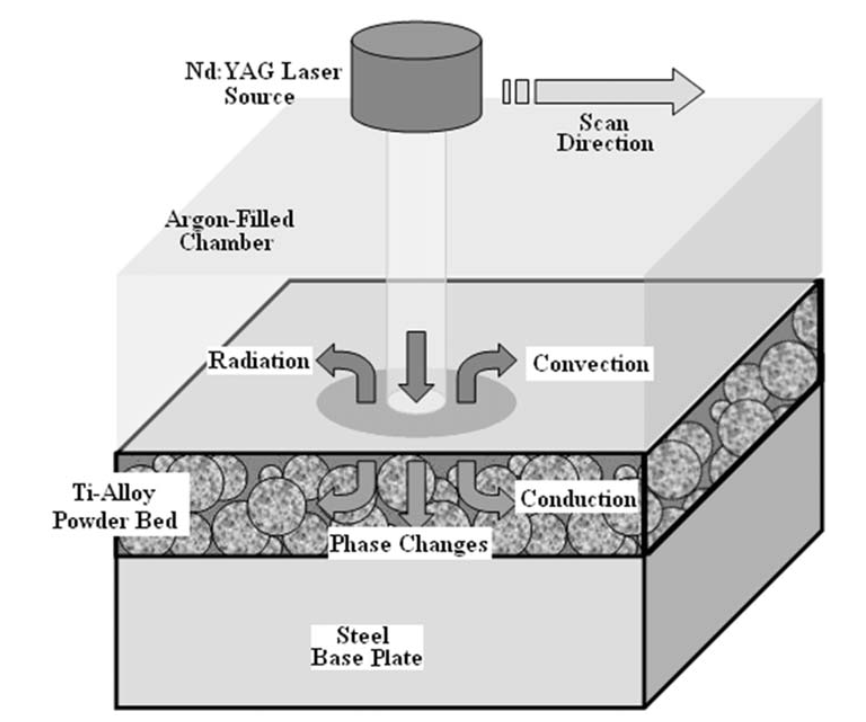
\includegraphics[width=0.4\textwidth]{schRepresentationHeatTransfer}
	\caption{Schematic representation of heat transfer \cite{Robertsthreedimensionalfiniteelement2009}}
	\label{fig:schRepresentationHeatTransfer}
\end{figure}

These phenomena have different effects on the process and can be split into two main groups : microscopic (focusing on the melting pool and the phase changement) and macroscopic (considering phenomena at the scale of the complete layer to build). A mesoscopic approach can then be run to link the two previous ones. (\cite{MegahedMetaladditivemanufacturingprocess2016,VanBelleAnalysemodelisationsimulation2013})

\section{Microscopic phenomena} 
The information about this part are mainly driven from \cite{DebRoyAdditivemanufacturingmetallic2018,MegahedMetaladditivemanufacturingprocess2016}
The microscopic model aims at representing what happends in the melting pool. The domain taken for this study is of a size comparable to the melting pool's one. In this model are considered :
\begin{itemize}
	\item heat source interaction with the feedstock,
	\item heat transfer (with high convection and radiation in the liquid phase),
	\item phase change (thermic parameters are modified depending on the temperature),
	\item surface tension forces,
	\item effect of thermal gradients leading to Marangoni forces,
	\item buoyancy.
\end{itemize}

\subsection{Model equations}

The notations here are $\rho$ the fluid density, $t$ is time, $\vec{\nu}$ the mass-averaged velocity vector, $p$ the hydrodynamic pressure, $\tau$ the deviatoric shear stress, $C$ a large constant, $f_L$ the liquid fraction and $f_v$ the vapor fraction while the phase is changing, $\sigma$ the surface tension, $\kappa$ the surface curvature, $\vec{n}$ the normal vector, $T$ the temperature, $p_R$ the recoil pressure, $\vec{g}$ the gravity vector, $h$ the total enthalpy and $h_i$ the specific enthalpy for the species $i$, $\lambda$ the conductivity, $\vec{j_i}$ the species mass flux, $L_f$ and $L_v$ the latent heat of fusion and evaporation, $S_r$ the term source representing radiation, $Y_i$ the species mass fraction, $m_L$ and $m_v$ the liquid and vapor mass sources due to phase change.

\vspace{0cm}

Different phenomena have to be modelised (equations from \cite{MegahedMetaladditivemanufacturingprocess2016}):

\begin{itemize}
	\item Mass conservation :
	\begin{equation}
	\partial_t\rho+\nabla.\rho \vec{\nu}=0
	\end{equation}
	
	\item Momentum conservation :
	\begin{equation}
	\partial_t(\rho\vec{\nu})+\nabla.\rho\vec{\nu}\vec{\nu}=-\nabla p+\nabla.\tau-\frac{C(1-f_L)^2}{f_L^3+10^{-10}}\vec{\nu}+\Big[\sigma\kappa\vec{n}+\frac{d\sigma}{dT}\Big(\nabla T-\vec{n}(\vec{n}.\nabla T)\Big)\Big]\cdot \vec{n}+p_R\cdot\vec{n}+\rho\vec{g}
	\end{equation}
	
	\item Energy conservation :
	\begin{equation}
	\partial_t(\rho h)+\nabla.\rho \vec{\nu}h=\nabla.\Big(\lambda\nabla T+\sum_ih_i\vec{j}_i\Big)+\partial_tp+\tau:\nabla\vec{\nu}-\partial_t(\rho f_LL_f)-\nabla(\rho\vec{\nu}f_LL_f)-\rho\partial_t((1-f_v)L_v)+S_R\cdot\vec{n}
	\end{equation}
	
	\item Species conservation :
	\begin{equation}
	\partial_t(\rho Y_i)+\nabla.\rho\vec{\nu}Y_i=\nabla.\vec{j}_i,\quad \forall i\in\llbracket1,N_{sp}\rrbracket
	\end{equation}
	
	\item Equation to track the free surface of the molten metal :
	\begin{equation}
	\partial_t\alpha_L+\nabla.\alpha_L\vec{\nu}=\frac{m_L}{\rho_L}-\frac{m_v}{\rho_L}
	\end{equation}
\end{itemize}


These equations can be simplified with some hypothesis. For exemple, in \cite{DebRoyAdditivemanufacturingmetallic2018}, they assume that there is no material losses by evaporation and that the liquid density stays constant in time. This lead to a new system of equations. (I haven't checked that they really correspond to the ones written above).


\subsection{To control}
Finally, let's explain why considering the microscopic scale is important. First of all, this enables a accurate description of the absorption of the heat source and thus gives an "equivalent" heat source for the macroscopic scale. Moreover, some defects come from the melting pool and the way the phase is changing. Some examples of these problems are presented here (see mainly \cite{DebRoyAdditivemanufacturingmetallic2018}).
\begin{itemize}
	\item Kevin Helmoltz instabilities
	\item Raleigh capillary instabilities
	\item loosing elements through evaporation
	\item porosity
	\item surface roughness
	\item damages...
\end{itemize}




\section{Macroscopic phenomena}

The macroscopic model "ignores" what happens in the melting pool. It considers more "global" effects and the domain size is the workingpiece one. The goal of this approach is to determine the residual stresses and distortion happening at the scale of the workpiece. To get this, a "two-scale" model is developed : first a heat transfer model whose results will be used for a mechanical analysis. 

\subsection{Heat transfer analysis}

In this model are considered :
\begin{itemize}
	\item the absorption of the heat source (modelized to void considering the melting pool)
	\item conduction in the solid
	\item radiation and convection
\end{itemize}

It is also assumed that the thermic parameters are constant over time and they don't depend on temperature but only of the fact that the represent powder or solid.

\subsubsection*{Model equations}

We note $\rho,\,\lambda,\,h,\,T,\,Q$ respectively the density, the conductivity, the enthalpy, the temperature and the inter volumic heat source. The parameter $c_p$ is the specific heat, that we assume constant over time (it only differs from solid to powder but the specific heat of powder and of solid stay constant over time). The ambiant temperature is $T_0$, $\beta(x)$ is the heat convection coefficient, $A$ the Hooke's operator. Finally, $\alpha$ is the thermal expansion coefficient, $f_{VonMises}$ the yield function and $\sigma_Y$ the yield stress.

\vspace{1cm}

The solid and the powder have different values for some physical parameters.
Thus, we consider here (for example with $\chi_{solid}$ the solid characteristic, $\rho_{solid}$ the density of the solid and $rho_{powder}$ the density of the powder):  (\cite{LiParametricanalysisthermal2014,Robertsthreedimensionalfiniteelement2009,AllaireTakingaccountthermal2017})
\begin{equation}
\begin{aligned}
\rho=\rho_{solid}*\chi_{solid}+\rho_{powder}*(1-\chi_{solid}) \\
c_p=c_{p,solid}*\chi_{solid}+c_{p,powder}*(1-\chi_{solid}) \\
\lambda=\lambda_{solid}*\chi_{solid}+\lambda_{powder}*(1-\chi_{solid}) \\
\epsilon=\epsilon_{solid}*\chi_{solid}+\epsilon_{powder}*(1-\chi_{solid}) \\
A=A_{solid}*\chi_{solid}+A_{powder}*(1-\chi_{solid}) \\
\beta=\beta_{solid}*\chi_{solid}+\beta_{powder}*(1-\chi_{solid}) \\
\end{aligned}
\end{equation}

The coefficient for the solid and the powder can sometimes be related (conductivity for example, considering the porousity of the powder).

\begin{itemize}
	\item equations in the workpiece (\cite{LiParametricanalysisthermal2014,Robertsthreedimensionalfiniteelement2009,AllaireTakingaccountthermal2017,MegahedMetaladditivemanufacturingprocess2016}): 
	\begin{equation}
	\label{eq:eqChaleurSimple}
	\rho(x)\partial_th(t,x)-\nabla(\lambda(x)\nabla T(t,x))=Q, \qquad \forall (t,x)\in (0,t_F)\times D
	\end{equation}	
	
	Specific heat and enthalpy are linked by (with $f_L$ the fraction of liquid and $L_f$ the latent heat) 
	\begin{equation}
	h=\int_{T_0}^{T}c_p(T)dT+f_LL_f
	\end{equation}
	
	Since the melting pool is ignored here and that the thermi parameters are considered constant over time, we get :
	\begin{equation}
	\rho(x)\partial_th(t,x)=\rho(x)c_p(x)\partial_tT(t,x)
	\end{equation}
	
	Thus the resulting equation is :
	\begin{equation}
	\rho c_p\partial_tT-div(\lambda\nabla T)=Q  \qquad  \textrm{in}\,\,(0,t_F)\times D 
	\end{equation}
	
	\item limit conditions (\cite{LiParametricanalysisthermal2014,Robertsthreedimensionalfiniteelement2009,MegahedMetaladditivemanufacturingprocess2016}):
	\begin{equation}
	\label{eq:conlimitemp}
	\left\{
	\begin{aligned}
	&(\lambda\nabla T)n=q-q_c-q_r \,\, \textrm{on}\,\, \partial D_N \\
	&T=T_0 \,\, \textrm{on}\,\,\partial D_D
	\end{aligned}
	\right.
	\end{equation}
	 
	with $q_c$ the heat convection (different from solid to powder), $q_r$ the heat radiation ($\sigma_B$ is the Stefan-Boltzman constant, $\epsilon$ is the emissivity), and $q$ is the heat source, considered as Gaussian here ($Ab$ is the absorptance, $P$ the laser power and $R$ the effective laser beam radius): 
	\begin{equation}
	\left\{
	\begin{array}{l}
	q_c=\beta (T-T_0)  \\
	q_r=\sigma_B\epsilon(T^4-T_0^4)	 \\
	q=\frac{2AbP}{\pi R^2}exp\Big(-\frac{2r^2}{R^2}\Big)
	\end{array}
	\right.
	\end{equation}
	
	 and the initial condition  
	 \begin{equation}
	 \label{eq:iniCondTemp}
	 T(x,y,z,0)=T_0 \,\, \forall x\in D
	 \end{equation}
	 
	 These boundary conditions are sumed up in Figure \ref{fig:BCSLM}:
	 
	 \begin{figure}
	 	\centering
	 	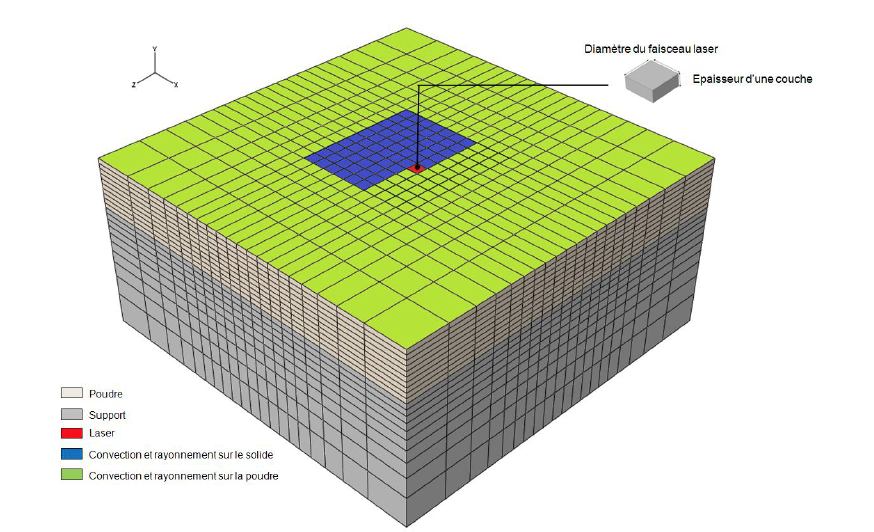
\includegraphics[width=0.7\textwidth]{BCSLM}
	 	\caption{}
	 	\label{fig:BCSLM}
	 \end{figure}
\end{itemize}

This leads to the following thermic problem :

\begin{equation}
\left\{
\begin{array}{ll}
\rho c_p\partial_tT-div(\lambda\nabla T)=Q  & \textrm{in}\,\,(0,t_F)\times D \\
(\lambda \nabla T)n=q-\beta (T-T_0)-\sigma_B\epsilon(T^4-T_0^4) & \textrm{on}\,\,(0,t_F)\times \partial D_N \\
T=T_0 &\textrm{on}\,\,(0,t_F)\times \partial D_D \\
T(x,y,z,0)=T_0 & \textrm{in}\,\,D
\end{array}
\right.
\end{equation}




	
\subsection{Thermo-mechanical analysis}

The mechanical analysis is non-linear. Depending on the loading applied and on the thermal load resulting from the laser scanning, plasticity can occur. We consider here a quasistatic model (\cite{MegahedMetaladditivemanufacturingprocess2016}) and the annealing effects are ignored.

\subsubsection*{Model equations}

\begin{equation}
\left\{
\begin{array}{l}
\nabla.\sigma+\vec{f}=0 \\
\epsilon^{tot}=\epsilon^e+\epsilon{th}+\epsilon^{p}\\
\sigma^e=C\epsilon^e=Ae(u^e) \\
\epsilon^{th}=\alpha(T-T_0)\\
\epsilon^{p}=f_{VonMises}(\sigma_Y)
\end{array}
\right.
\end{equation}

Boundary conditions are added to the problem :
\begin{equation}
\left\{
\begin{array}{ll}
\sigma\vec{n}=0 & \textrm{on\,}\partial D_N \\
u=0 & \textrm{on\,}\partial D_D
\end{array}
\right.
\end{equation}

\subsection{To control}
Different variables have to be controlled (\cite{DebRoyAdditivemanufacturingmetallic2018}):

\begin{itemize} 
	\item thermal stress : to avoid plasticity and thus residual constraints, the thermal stress must stay low.
	\item spatial thermic gradient : this one could also cause residual stresses and must be kept low too.
\end{itemize}



\section{Model for now}
A first model has been chosen to simplify the computation and to be taken as a working basis. This is basically the one taken in \cite{AllaireTakingaccountthermal2017}.

\subsection{Model in 2D, for only one layer}

\begin{equation}
\left\{
\begin{array}{ll}
\rho c_p\partial_tT-div(\lambda\nabla T)+\lambda T=q_{source}  & \textrm{in}\,\,(0,t_F)\times D \\
(\lambda \nabla T)n=-\beta (T-T_0) & \textrm{on}\,\,(0,t_F)\times \partial D_N \\
T=T_0 &\textrm{on}\,\,(0,t_F)\times \partial D_D \\
T(x,y,z,0)=T_0 & \textrm{in}\,\,D
\end{array}
\right.
\end{equation}

\begin{equation}
\label{eq:elastoplasticSystem}
\left\{
\begin{array}{ll}
-div(\sigma)=f & \textrm{in}\,(0,t_F)\times D \\
\sigma=\sigma^{el}+\sigma^{th} & \textrm{in}\,(0,t_F)\times D \\
\sigma^{el}=Ae(u)\quad \sigma^{th}=K(T-T_0)I_n \\
\sigma.n=0 & \textrm{on}\,(0,t_F)\times \partial D_N \\
u=0 & \textrm{on}\,(0,t_F)\times D_D \\
\end{array}
\right.
\end{equation}

\subsection{Model in 3D, for more than one layer}

\bibliographystyle{plain-fr}
\bibliography{biblio}

\end{document}
